\chapter[Alternate Heading Title]{Chapter Title}

\textbf{Disclaimer: This is not an official template and it does not follow any specific guidelines. Please confirm that it is suitable for your project before using it.}

\section{Research Question Formatting}

Donec\footnote{Example footnote} vel pellentesque quam, at pharetra ipsum. Vestibulum ipsum elit, condimentum id molestie eget, commodo at dui. Donec id laoreet tellus, a interdum urna. Duis fermentum lorem neque, sed iaculis magna laoreet placerat. Pellentesque convallis efficitur sollicitudin. Cras eu ipsum eget orci tincidunt porttitor vulputate id lacus. Praesent tincidunt finibus nulla, a viverra quam convallis a. In elementum commodo egestas.

\begin{center}
    \textit{How does X affect Y?}
\end{center}

\section{Citations}

The most notable work in Reinforcment Learning is that of Temporal Difference Learning \autocite{sutton_learning_1988}. Or cite in text: The work of \textcite{sutton_learning_1988} is the most ...

\section{Equations}

See Equation~\ref{eq:equation1}. Or inline equations with $y = mx + b$.

\begin{equation}
    G_t^\lambda = (1-\lambda) \sum_{n=1}^{T-t-1} \lambda^{n-1} G_{t:t+n} + \lambda^{T-t-1} G_{t:T}
    \label{eq:equation1}
\end{equation}

\clearpage

\section{Figures}

Figure~\ref{fig:figure1}, shows a basic figure.

\begin{figure}[htb]
    \centering
    \includegraphics[width=0.2\textwidth]{assets/2d.png}
    \caption{Figure caption}
    \label{fig:figure1}
\end{figure}

\begin{figure}[htb]
    \centering
    \begin{subfigure}[t]{0.2\textwidth}
        \centering
        \includegraphics[width=\textwidth]{assets/2d.png}
        \caption{Subfigure 1}
    \end{subfigure}
    \hspace{1cm}
    \begin{subfigure}[t]{0.20\textwidth}
        \centering
        \includegraphics[width=\textwidth]{assets/3d.png}
        \caption{rubfigure 2}
    \end{subfigure}
    \caption{Figure with subfigures}
\end{figure}

\clearpage

\subsection{Inline Figure}

\begin{wrapfigure}{r}{0.45\textwidth}
    \centering
    \includegraphics[width=0.45\textwidth]{assets/3d.png}
    \caption[Alternate Figure Title]{Sed hendrerit dui elit, non semper dolor consectetur eget. Fusce dignissim tellus a hendrerit posuere. Pellentesque imperdiet pulvinar orci, in tempor dui rutrum at. Duis porttitor porttitor dolor, sit amet imperdiet erat venenatis nec. Donec vehicula quam vitae mi fermentum, nec vehicula ligula viverra. Proin consequat suscipit arcu nec semper. In quis turpis nec mi tristique euismod sed nec eros. Donec laoreet facilisis tellus sit amet rhoncus. Proin eu ligula massa. Morbi tristique enim nunc}
    \label{fig:inline}
\end{wrapfigure}

Lorem ipsum dolor sit amet, consectetur adipiscing elit. Donec convallis pharetra nunc vel congue. Phasellus nisi nunc, semper in purus vitae, dapibus ultrices nisi. Proin sagittis elementum mi. Cras blandit metus eu tortor suscipit vulputate. Morbi suscipit molestie tristique. Pellentesque aliquam dapibus risus, in vestibulum justo molestie et. Integer sit amet viverra est, ut imperdiet purus. Integer aliquam hendrerit sem, et porta massa volutpat eu.

Sed hendrerit dui elit, non semper dolor consectetur eget. Fusce dignissim tellus a hendrerit posuere. Pellentesque imperdiet pulvinar orci, in tempor dui rutrum at. Duis porttitor porttitor dolor, sit amet imperdiet erat venenatis nec. Donec vehicula quam vitae mi fermentum, nec vehicula ligula viverra. Proin consequat suscipit arcu nec semper. In quis turpis nec mi tristique euismod sed nec eros. Donec laoreet facilisis tellus sit amet rhoncus. Sed tristique velit ac nibh malesuada semper. Vestibulum venenatis sem sit amet quam egestas, non eleifend sem venenatis. Proin eu ligula massa. Morbi tristique enim nunc, a imperdiet lorem volutpat et.

Fusce facilisis sit amet sapien non molestie. Maecenas magna arcu, ultrices nec sollicitudin sed, tristique a eros. Ut rutrum gravida purus, eu posuere mi tincidunt sit amet. Praesent sed egestas est. Maecenas scelerisque quis sapien eu lobortis. Mauris id nisl ac sapien dictum efficitur in vitae arcu. Ut sagittis tempus magna sed egestas. Maecenas tempor nec odio sit amet molestie. Maecenas sagittis egestas arcu a cursus. Vivamus in orci at sapien cursus tempor sed vitae tortor. Curabitur nec augue nisl. Nam congue nisi ornare, mattis dui quis, vestibulum dui.

Nullam vitae arcu commodo, accumsan odio et, sollicitudin elit. Quisque enim est, placerat et fermentum non, mollis et turpis. Nunc risus neque, congue in tortor et, rutrum ultrices urna. Vivamus quis lorem volutpat, suscipit leo sed, gravida orci. Nullam varius nisl sit amet nibh congue gravida. Quisque ut leo dapibus, rutrum mi nec, luctus dui. Fusce eros erat, tempor ac tempus in, lobortis vel tellus. Quisque et neque neque. Maecenas tincidunt lacus et nisl finibus efficitur. Aliquam bibendum vitae sem auctor luctus. Nulla hendrerit lorem convallis convallis tempus. Class aptent taciti sociosqu ad litora torquent per conubia nostra, per inceptos himenaeos.

\subsection{Tikz}

\begin{figure}[htb]
    \centering
    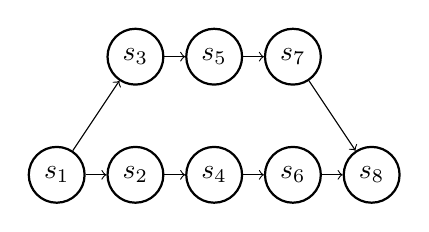
\begin{tikzpicture}
        \tikzstyle{state}=[circle,draw=black,thick,minimum size=0.5cm]
        \node[state] (s1) at (0,0) {$s_1$};
        \node[state] (s2) at (1,0) {$s_2$};
        \node[state] (s3) at (2,0) {$s_4$};
        \node[state] (s4) at (1,1.5) {$s_3$};
        \node[state] (s5) at (3,0) {$s_6$};

        \node[state] (s6) at (4,0) {$s_8$};
        \node[state] (s7) at (2,1.5) {$s_5$};
        \node[state] (s8) at (3,1.5) {$s_7$};

        \draw[->] (s1) -- (s2);
        \draw[->] (s1) -- (s4);
        \draw[->] (s2) -- (s3);
        \draw[->] (s3) -- (s5);
        \draw[->] (s4) -- (s7);
        \draw[->] (s5) -- (s6);
        \draw[->] (s7) -- (s8);
        \draw[->] (s8) -- (s6);
    \end{tikzpicture}
    \caption{A Tikz figure}
    \label{fig:tikz}
\end{figure}

\section{Tables}

\begin{table}[htb]
    \centering
    \caption{Table caption usually above the table}
    \label{tab:environments}
    \resizebox{0.3\textwidth}{!}{%
        \begin{tabular}{@{}lll@{}}
            \toprule
            Name     & Type     & Top Speed \\ \midrule
            Audi     & Sport    & 200       \\
            BMW      & Comfort  & 160       \\
            Tesla    & Electric & 170       \\
            Mercedes & Comfort  & 170       \\ \bottomrule
        \end{tabular}%
    }
\end{table}

\section{Code}

\begin{algorithm}
    \caption{Algorithm caption}
    \begin{algorithmic}[1]
        \State $w \gets 0$ \Comment{$w$ is a column vector of size $|\mathcal{S}|$}
        \State $\mathbf{M} \gets 0$ \Comment{$\mathbf{M}$ is a matrix of size $|\mathcal{S}| \times |\mathcal{S}|$}
        \For {each episode}
        \State $e \gets 0$
        \For {each $s$, $s^\prime$ and $r$ of episode}
        \State $e(s) \gets e(s) + 1$ \Comment{Tabular accumulating trace}
        \State $\mathbf{M} \gets \mathbf{M}  + \beta e \mathbf{s}^\top + \beta \gamma e \mathbf{s}^{\prime\top} \mathbf{M} - \beta e \mathbf{s}^{\top} \mathbf{M} $ \Comment{$\mathbf{s}$, $\mathbf{s^\prime}$ in bold marks the state as one-hot vector $|\mathcal{S}|$}
        \State $\delta \gets r + \gamma v_w(s^\prime) - v_w(s)$
        \State $w \gets w + \alpha \mathbf{M} \mathbf{s} \delta$
        \State $e \gets \gamma \lambda e$
        \EndFor
        \EndFor
        \State \Return $w$
    \end{algorithmic}
\end{algorithm}
